%% ------------------------------------------------------------------------- %%
\chapter{Theoretical Background}
\label{cap:conceitos}
In this chapter, the theoretical concepts that apply to this research are stated. First, a short introduction to color models is provided in order to give an overview of the main characteristics of some of the most used in the computer vision and image processing area, on which this research is based. Thereafter, some machine learning methods are defined and explained, once they were used in the preliminary experiments of this work.                                                                                                                               

%% ------------------------------------------------------------------------- %%
\section{Color models}
\label{sec:fundamentos}

The use of color images in computer vision or image processing can be motivated by two main factors. The first refers to the powerful characteristic of color to function as a descriptor that often simplifies the identification and extraction of an object in a scene. The second is related to the ability of humans to discern thousands of tonalities and intensities compared to only a few dozen levels of gray \citep{gonzalez:02}.

The visual perception of color by the human eye should not vary according to the spectral distribution of the natural light incident upon an object. In other words, the color appearance of objects remains stable under different lighting conditions. This phenomenon is known as color constancy \citep{gevers:12}.

As an example, the grass of a soccer stadium remains green throughout the day, even at dusk when, from a physical point of view, sunlight has a more reddish appearance.

The human perception of colors occurs by the activation of nerve cells that send signals to the brain about brightness, hue and saturation, which are usually the features used to distinguish one color from another \citep{gonzalez:02}.

The brightness gives the notion of chromatic intensity. Hue represents the dominant color perceived by an observer. Saturation refers to the relative purity or amount of white light applied to the hue. Combined, hue and saturation are known as chromaticity and, therefore, a color must be characterized by its brightness and chromaticity \citep{gonzalez:02}.

Colors can be specified by mathematical models in tuples of numbers in a coordinate system and a subspace within that system where each color is represented by a single point. Such models are known as the color models \citep{gonzalez:02}.

These models can be classified as of two types: the additive models in which the primary color intensities are added to produce other colors and subtractive, where colors are generated by subtracting the length of the dominant wave from the white light.

The following sections briefly describe some of the major color models, as well as their variants and main areas of application.

%% ------------------------------------------------------------------------- %%
\subsection{Munsell color model}
\label{sec:modelo_cores_munsell}

Pioneer in an attempt to organize the perception of color in a color space, Albert H. Munsell was able to combine the art and science of colors in a single theory \citep{konstantinos:00}.

The principle of equality of visual spacing between the components of the model is the essential idea of the Munsell color model. These components are hue, value, corresponding to luminance, and chroma, corresponding to saturation \citep{konstantinos:00}.

The model is represented by a cylindrical shape and it can be seen in the figure ~\ref{fig:munsell-system}. The hue is arranged in the circular axis consisting of five base as well as five secondary colors, the saturation in the radial axis and the luminance in the vertical axis in a range varying from 0 to 10.

\begin{figure}[!h]
  \centering
  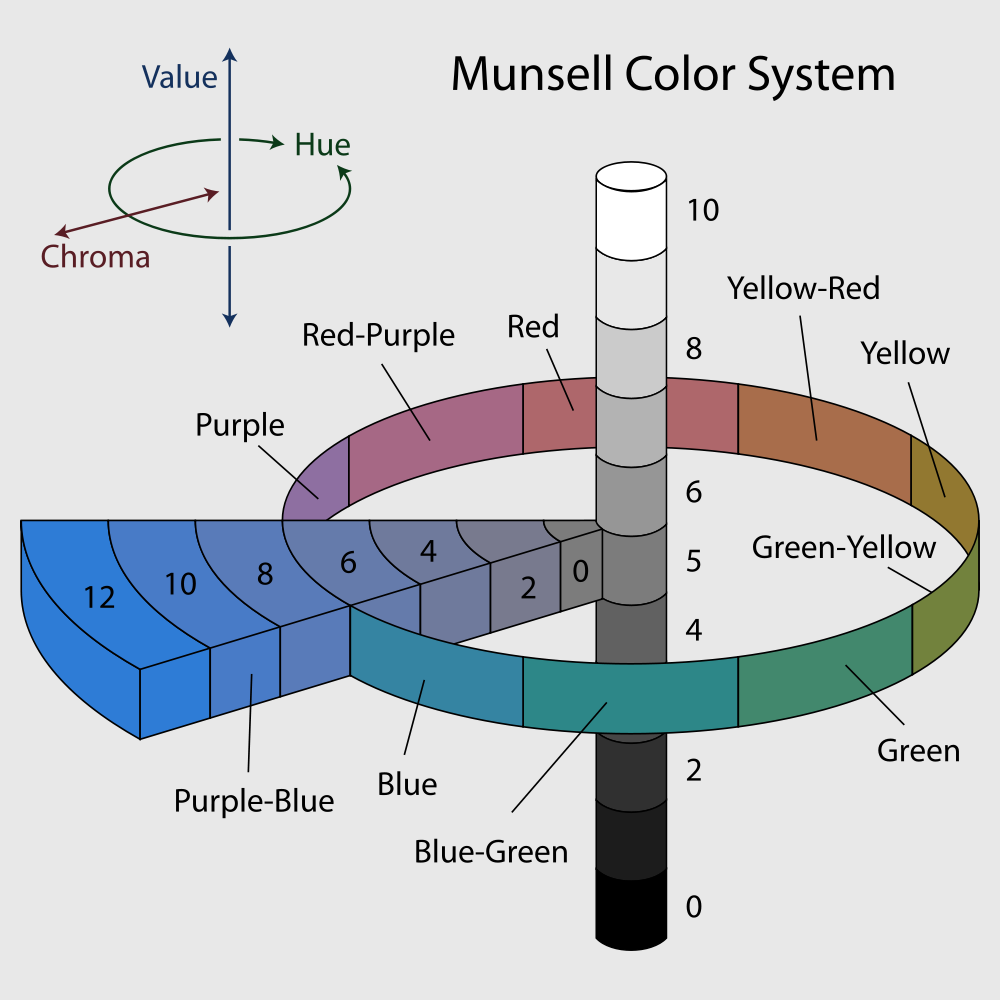
\includegraphics[width=.55\textwidth]{munsell-system}
  % fonte https://commons.wikimedia.org/wiki/File:Munsell-system.svg
  \caption[Munsell color model.]{Munsell color model represented by a cylindrical shape. The hue is arranged on the circular axis consisting of five base and five secondary colors, the saturation on the radial axis and the luminance on the vertical axis in a range varying from 0 to 10. Source: \citet{rus:07}.}
  \label{fig:munsell-system} 
\end{figure}

%% ------------------------------------------------------------------------- %%
\subsection{CIE color model}
\label{sec:modelo_cores_cie}

In 1931, the CIE established the first mathematical model of color numerical specification, whose objective was to analyze the relationship between the physical aspects of colors in the electromagnetic spectrum and their perception by the human visual system to determine how an ordinary person perceives the color. A review of this specification was published in 1964 \citep{gonzalez:02}.

The experiment that originated the standard consisted in detecting the colors perceived by an observer from a mixture of three primary colors X, Y and Z called tristimulus values. These coordinates gave rise to the CIE XYZ color space which encompasses all the colors that can be perceived by an ordinary human being. For this reason, it is considered an device independent representation \citep{konstantinos:00}.

The system proposed by the CIE XYZ to describe a color is based on a luminance component Y, and two additional components X and Z, that bring the chromaticity information. This system is formed by imaginary colors that can be expressed as combinations of the normalized measures shown in the equations~\ref{eq:cie_x}, \ref{eq:cie_y} and \ref{eq:cie_z}.

\begin{equation}
  x = \frac{X}{X + Y + Z}
\label{eq:cie_x}
\end{equation}

\begin{equation}
  y = \frac{Y}{X + Y + Z}
\label{eq:cie_y}
\end{equation}

\begin{equation}
  z = \frac{Z}{X + Y + Z}
\label{eq:cie_z}
\end{equation}

where $x + y+ z = 1$.

Combinations of negative values and other problems related to selecting a set of real primaries are eliminated. The chromaticity coordinates $x$ and $y$ allow to represent all colors in a two-dimensional plane, also known as a chromaticity diagram, which can be seen in the figure ~\ref{fig:cie-cromaticity-diagram}.

\begin{figure}[!h]
  \centering
  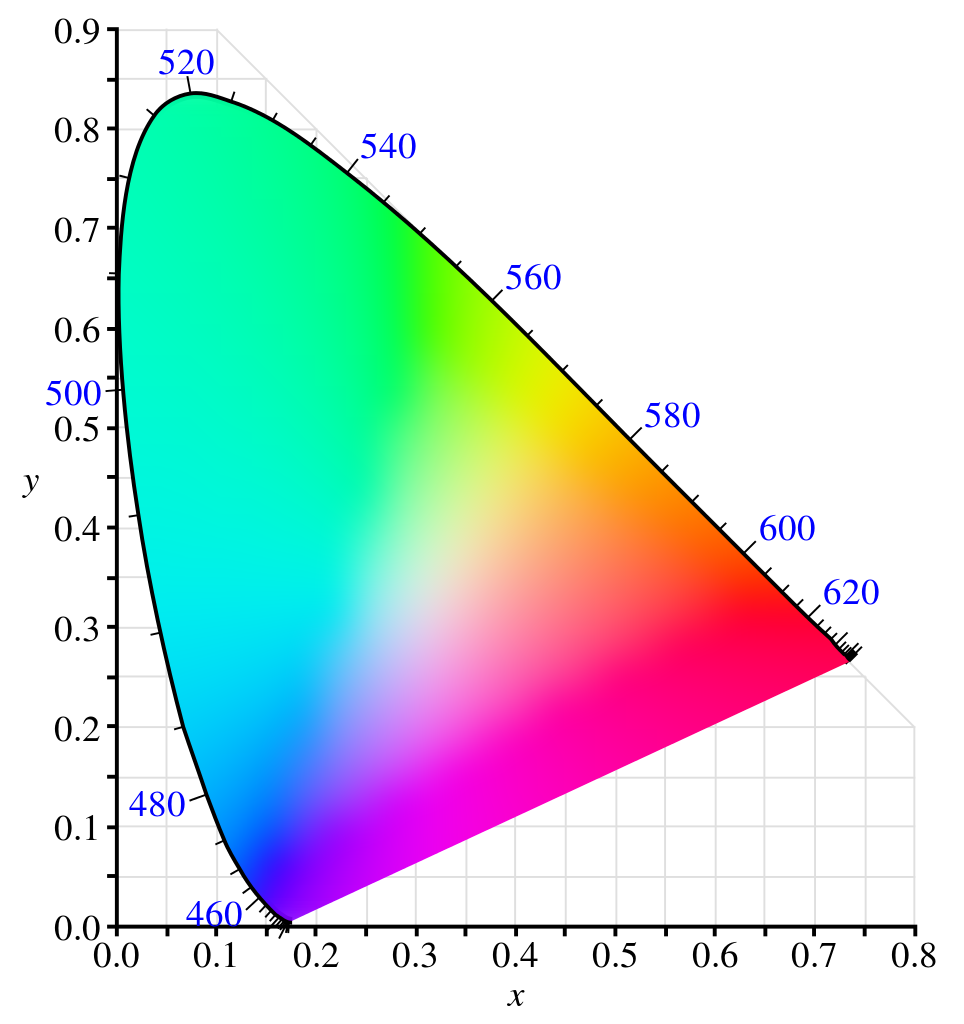
\includegraphics[width=.5\textwidth]{cie-cromaticity-diagram}
  % fonte https://en.wikipedia.org/wiki/File:CIE1931xy_blank.svg
  \caption[CIE 1931 chromaticity diagram]{CIE 1931 chromaticity diagram. The points representing pure colors in the electromagnetic spectrum are labeled according to their wavelengths and are located along the curve from the right end of the x-axis, corresponding to the red color, to the left end of the same axis, corresponding to the violet color, forming a polygon similar to a horseshoe. The internal points correspond to all possible combinations of visible colors. Source: \citet{ben:09}.}
  \label{fig:cie-cromaticity-diagram} 
\end{figure}

The coordinates $ (x = 1/3, y = 1/3) $ correspond to the location of white light, also known as white point, and serve as reference in the process of image capture, coding, or reproduction.

CIE also derived and standardized two other color models based on CIE XYZ specification and, likewise, are device independent. Both are perceptually uniform, which means that equal perceptual distances separate all colors in the system~\citep{vezhnevets:03}. As an example, the gray scale of the space should allow for a smooth transition between black and white.

The first one was designed to reduce the problem of perceptual non-uniformity. Some Uniform Chromaticity Scale (UCS) diagrams were proposed based on mathematical equations to transform the values XYZ or the coordinates $x, y$ into a new set of values $(u, v)$, which gave rise to the 1960 CIE $uv$ chromaticity diagram~\citep{gevers:12}.

Still with unsatisfactory results, the CIE made a new change by multiplying the $v$ component by a factor of 1.5. In addition, the brightness scale given by the Y component has been replaced by $L^* = [0, 100]$ to better represent the differences in luminosity that are equivalent. This revision originated the CIE 1976 $L^*u^*v^*$ color model, commonly known by the acronym CIELuv~\citep{gevers:12}.

In 1976 the CIE adopted a new color model, based on the $L, a, b$ model, proposed by Richard Hunter in 1948, which best represented the uniform spacing of colors. Named CIE $L^*a^*b^*$ and known by the acronym CIELab, it is a space based on opponent colors \footnote{Theory started around 1500 when Leonardo da Vinci concluded that colors are produced by mixing yellow and blue, green and red, and white and black. In 1950, this theory was confirmed when optically-colored signals were detected at the optical connection between the retina and the brain~\citep{gevers:12}.} in which the color stimuli of retina is converted to distinctions between light and dark, red and green, and blue and yellow, represented by the axes $L^*$, $a^*$, and $b^*$, respectively~\citep{gevers:12}.


%% ------------------------------------------------------------------------- %%
\subsection{RGB color model}
\label{sec:modelo_cores_rgb}

The RGB model, an acronym for Red, Green, and Blue, is an additive color model in which the three primary colors red, green and blue are added to produce the others \citep{gonzalez:02}.

This system was based on the trichromatic theory of Thomas Young and Hermann Helmholtz in the mid-19th century and can be represented graphically
through the unit cube defined on the axes R, G and B, as illustrated in the figure~\ref{fig:rgb-cube} \citep{konstantinos:00}.

\begin{figure}[!h]
  \centering
  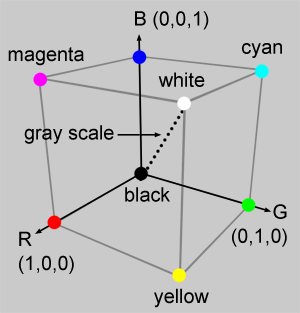
\includegraphics[width=.35\textwidth]{rgb-cube}
  % http://www.scratchapixel.com/old/lessons/3d-basic-lessons/lesson-5-colors-and-digital-images/color-spaces/
  \caption[Unit cube representing the colors of the RGB model]{Unit cube representing the colors of the RGB model. The origin, given by the vertex $(0, 0, 0)$, represents the black color. The vertex $(1, 1, 1)$, opposite the origin, represents the white color. The highlighted vertices on the axes represent the primary colors and the others are the complement of each. Each point inside the cube corresponds to a color that can be represented by the triple $(r, g, b)$, where $r, g, b \in [0, 1]$. The shades of gray are represented along the main diagonal of the cube, with each point along this diagonal being formed by equal contributions of each primary color. Source: adapted from \citet{gonzalez:02}.}
  \label{fig:rgb-cube} 
\end{figure}

It is noteworthy that there are two ways of representing the RGB space: linear and non-linear. The above-mentioned system shows the non-linear model, whose abbreviation is $R'G'B'$, and is most used by devices and applications because of their similarity to the human visual system. In the literature, this system is frequently cited with the acronym RGB, which makes the nomenclature dubious, since the linear model is also called RGB and, therefore, the conversion between color spaces must be done with some caution. It is also important to note that linear RGB values are rarely used to represent an image since they are perceptually highly non-uniform \citep{konstantinos:00}.


%% ------------------------------------------------------------------------- %%
\subsection{CMY color model}
\label{sec:modelo_cores_cmy}

The CMY model is based on the complementary primary colors Cyan, Magenta, and Yellow and, unlike RGB, is a subtractive color model in which colors are generated by subtracting the length of the dominant wave from the white light and, therefore, the resulting color corresponds to the light that is reflected \citep{gonzalez:02}.

One way to get the CMY system is:\\
\begin{equation}
  \begin{bmatrix}
    C \\ M \\ Y
  \end{bmatrix} = 
  \begin{bmatrix}
    B \\ R \\ R
  \end{bmatrix} +
  \begin{bmatrix}
    G \\ B \\ G
  \end{bmatrix}
\end{equation}

\noindent or by making a change of coordinates by subtracting the primary colors R, G and B of the white color $W = (1, 1, 1)$ \citep{gonzalez:02}:
\begin{equation}
  \begin{bmatrix}
    C \\ M \\ Y
  \end{bmatrix} = 
  \begin{bmatrix}
    1 \\ 1 \\ 1
  \end{bmatrix} -
  \begin{bmatrix}
    R \\ G \\ B
  \end{bmatrix}
\end{equation}

Likely RGB, CMY is device dependent. The model is widely used in equipment that deposits colored pigments on paper, such as color printers or photocopiers. The figure~\ref{fig:cmy-model} shows how the model components are combined to generate the other colors.

\begin{figure}[!h]
  \centering
  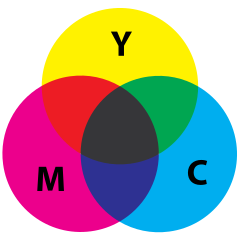
\includegraphics[width=.25\textwidth]{cmy-model}
  % https://en.wikipedia.org/wiki/File:SubtractiveColor.svg
  \caption[CMY subtractive color model]{CMY subtractive color model. It is interesting to note that the intersection of yellow with magenta generates the red color, magenta with cyan generates the blue color and cyan with yellow generates the green color. Source: \citet{rus:08}.}
  \label{fig:cmy-model}
\end{figure}

Overlapping the CMY primary colors in equal amounts to generate the black color typically creates a tint that is close to brown or dark green. To avoid this undesired effect, the black component is usually added to the system, represented by the letter K. This operation gives rise to a new model known as \textbf{CMYK}~\citep{gonzalez:02}.

%% ------------------------------------------------------------------------- %%
\subsection{Color models of the YUV family}
\label{sec:modelo_cores_yuv}

The acronym YUV stands to a family of color spaces of which the luminance information, represented by the Y component, is coded separately from the chrominance, given by the components U and V. The components U and V are representations of signals of the difference of the blue subtracted from luminance (B-Y) and red subtracted from luminance (R-Y). It is used to represent colors in analogue television transmission systems in the Phase Alternating Line (PAL) and Sequential Color with Memory (SECAM)~\citep{pedrini:08}.

The transformation of the RGB space to YUV is given by:\\
\begin{equation}
  \begin{bmatrix}
    Y \\ U \\ V
  \end{bmatrix} = 
  \begin{bmatrix}
     0.299 &  0.587 &  0.114 \\
    -0.147 & -0.289 &  0.436 \\
     0.615 & -0.515 & -0.100 \\
  \end{bmatrix}
  \begin{bmatrix}
    R \\ G \\ B
  \end{bmatrix}
\end{equation}
where $0 \leq R, G, B \leq 1$.

Analogous to the YUV, the YIQ model was adopted in 1950 by the National Television System Committee (NTSC), an American standard for color television signal transmission. In this model, the Y component corresponds to luminance and the components I (hue) and Q (saturation) encode the chrominance information \citep{pedrini:08}.

The transformation of the RGB space to YIQ is given by:\\
\begin{equation}
  \begin{bmatrix}
    Y \\ I \\ Q
  \end{bmatrix} = 
  \begin{bmatrix}
    0.299  &  0.587 &  0.114 \\
    0.596  & -0.275 & -0.321 \\
    0.212  & -0.523 & -0.311 \\
  \end{bmatrix}
  \begin{bmatrix}
    R \\ G \\ B
  \end{bmatrix}
\end{equation}
where $0 \leq R, G, B \leq 1$.

Another color model of the YUV family is the YCbCr, mathematically defined by a coordinate transformation with respect to some RGB space~\citep{pedrini:08}.

The YCbCr model is widely used in digital videos. In this system, the Y component represents luminance, Cb component gives the measurement of the difference between the blue color and a reference value, similar to the Cr component which is the measurement of the difference between the red color and a reference value~\citep{pedrini:08}.

The transformation of the RGB space to YCbCr is given by:\\
\begin{equation}
  \begin{bmatrix}
    Y \\ Cb \\ Cr
  \end{bmatrix} = 
  \begin{bmatrix}
     0.299 &  0.587 &  0.114 \\
    -0.169 & -0.331 &  0.5   \\
     0.5   & -0.419 & -0.081 \\
  \end{bmatrix}
  \begin{bmatrix}
    R \\ G \\ B
  \end{bmatrix}
\end{equation}


%% ------------------------------------------------------------------------- %%
\subsection{Color models of the HSI family}
\label{sec:modelo_cores_hsi}

Hue, Saturation, and Intensity (HSI) models are best suited for image processing applications from the user's point of view, due the correlation with human perception of the color~\citep{konstantinos:00}.

In this model, as in YIQ, the intensity given by I component is decomposed from the chrominance information, represented by the hue (H) and saturation (S) \citep{konstantinos:00}. The combination of these components results in a pyramidal structure which can be seen in figure~\ref{fig:hsi-model}.

\begin{figure}[!h]
  \centering
  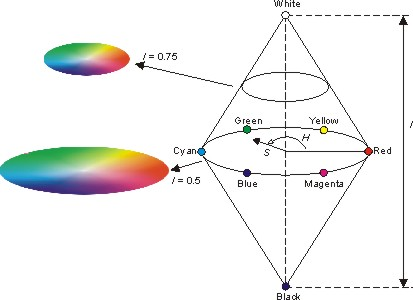
\includegraphics[width=.7\textwidth]{hsi-model}
  % http://www.blackice.com/images/HSIColorModel.jpg
  \caption[Graphical representation of the HSI model]{Graphical representation of the HSI model. The hue describes the color itself, in the form of an angle $\theta$, where $\theta \in [0, 360]$. Red is at 0 degree, yellow at 60, green at 120, and so on. The saturation component, which varies between 0 and 1, indicates how much color is polluted with white color. The intensity scale is between $[0, 1]$, where 0 means black and 1, white. Source: \citet{blackice:16}.}
  \label{fig:hsi-model} 
\end{figure}

The transformation of the components of the RGB space to HSI is given by the equations:
\begin{align}
\label{eq:rgb_para_hsi}
\begin{split}
  \theta &= cos^{-1} \bigg( \frac{(R - G) + (R - B)}{2 \sqrt{(R - G)^2 + (R - B)(G - B)}} \bigg)
  \\[0.5em]
  H &= \begin{cases}
            \theta,       & \text{if}\ B \leq G\\
            360 - \theta, & \text{otherwise}\\
       \end{cases}
  \\[0.5em]
  S &= 1 - \frac{3 min(R, G, B)}{R + G + B}
  \\[0.5em]
  I &= \frac{R + G + B}{3}
\end{split}
\end{align}

It is important to note that the values R, G and B must be normalized in the interval between 0 and 1. The intensity $I$ and the saturation $S$ are also normalized between 0 and 1.

Another model of this family is formed by the components Hue, Saturation and Value (HSV) and its three-dimensional graphical representation is a hexagonal pyramid derived from the RGB cube \citep{pedrini:08}. Value, in this context, is the luminance component.

The various hue shades are represented at the top of the pyramid, the saturation is measured along the horizontal axis and value is measured along the vertical axis, which passes through the center of the pyramid. The hue, which corresponds to the edges around the vertical axis, varies from 0 (red) to 360 degrees and the angle between the vertices is 60 degrees. The saturation varies from 0 to 1 and is represented as the ratio of the purity of a given hue to its maximum purity, that is, when $S = 1$. Value varies from 0, at the peak of the pyramid representing the black color, to 1 at the base, where the intensities of the colors are maximum~\citep{pedrini:08}.

The transformation of the components of the RGB space to HSV is given by the equations:
\begin{align}
\label{eq:rgb_para_hsv}
\begin{split}
  H &=  \begin{cases}
            60\ffrac{(G - B)}{M - m}, & \text{if}\ M = R\\[0.7em]
            60\ffrac{(B - R)}{M - m} + 120, & \text{if}\ M = G\\[0.7em]
            60\ffrac{(R - G)}{M - m} + 240, & \text{if}\ M = B
       \end{cases}
  \\[0.5em]
  S &=  \begin{cases}
            \ffrac{(M - m)}{M}, \quad &\text{if}\ M \neq 0\\[0.7em]
            0, \quad &\text{otherwise}\\
       \end{cases}
  \\[0.5em]
  V &= M
\end{split}
\end{align}

\noindent where $m = min(R, G ,B)$ and $M = max(R, G ,B)$. The luminance $V$ and saturation $S$ are normalized between 0 and 1. The $H$ hue ranges from 0 to 360 degrees.

Similarly to HSV, the Hue, Saturation and Lightness (HSL) model is a three-dimensional representation and is formed by two cones of height 1, whose bases are coincident \citep{pedrini:08}.

The hue is determined by the points in the circle of the common bases to the cones. The saturation varies from 0 to 1, depending on the distance to the axis of the cone. The lightness is along the vertical axis common to the two cones and varies in the scale $[0, 1]$, where 0 means black and 1, white \citep{pedrini:08}.

The conversion of the RGB space to HSL is given by the equations:
\begin{align}
\label{eq:rgb_para_hsl}
\begin{split}
  H &=  \begin{cases}
            60\ffrac{(G - B)}{M - m}, & \text{if}\ M = R\\[0.7em]
            60\ffrac{(B - R)}{M - m} + 120, & \text{if}\ M = G\\[0.7em]
            60\ffrac{(R - G)}{M - m} + 240, & \text{if}\ M = B
       \end{cases}
  \\[0.5em]
  S &=  \begin{cases}
            \ffrac{(M - m)}{M + m}, & \text{if}\ 0 < L \leq 0,5\\[0.7em]
            \ffrac{(M - m)}{2 - (M + m)}, & \text{if}\ L > 0,5\\[0.5em]
            0, & \text{if}\ M = m\\
       \end{cases}
  \\[0.5em]
  L &= \frac{M + m}{2}
\end{split}
\end{align}

\noindent where $m = min(R, G ,B)$ and $M = max(R, G ,B)$. The lightness $V$ and saturation $S$ are normalized between 0 and 1. Note that the transformation of the $H$ component is the same as that used in the conversion of the RGB to HSV space in \ref{eq:rgb_para_hsv} and varies between 0 and 360 degrees.

All the color models of this family have the property of thinking of lighter colors, obtained by increasing the brightness or lightness, and darker colors, by the diminution of the same values. The intermediate colors are produced by decreasing the saturation~\citep{pedrini:08}.


%% ------------------------------------------------------------------------- %%
\section{Classificadores}
\label{sec:classificadores}
A aprendizagem de máquina é uma área que está preocupada com o desenvolvimento de programas de computador capazes de melhorar automaticamente com a experiência \citep{mitchell:97}. Essa definição está intimamente ligada ao modo com que seres humanos aprendem. Os esforços de pesquisa nessa área têm sido realizados com o propósito de aproximar esta relação.

Como exemplo, ao mostrar a imagem de uma árvore para uma criança de três anos de idade, muito provavelmente ela saberá reconhecê-la, pois deve ter sido exposta a situações em que tenha visto imagens semelhantes e, sendo assim, foi treinada para dar tal resposta. Logo, ela aprendeu o que é uma árvore apenas olhando para elas, não necessariamente por meio de definições matemáticas precisas. Em outras palavras, o aprendizado foi feito com base em dados que, muitas vezes, são utilizados para obter-se soluções empíricas para determinados problemas onde não há a possibilidade de se criar uma solução analítica \citep{mostafa:12}.

Analogamente, um algoritmo pode ser treinado para diferenciar uma árvore de outros objetos com base em um conjunto de dados que possui descrições sobre as árvores, tais como, altura, cores, espessura, comprimento, etc. Tais descrições também são chamadas de atributos, propriedades ou características e são submetidas a um classificador que avalia as evidências apresentadas e toma uma decisão sobre o objeto sendo analisado \citep{duda:12}. Essa tarefa começa com a definição de um vetor de características em um espaço $d$-dimensional, da forma \citep{duda:12}:

\begin{equation}
\label{eq:vetor_caracteristicas}
  x = 
  \begin{bmatrix}
    a_1 \\ a_2 \\ \vdots \\ a_d
  \end{bmatrix}
\end{equation}
\noindent onde $x \in X$ e $X$ é o espaço de entrada, ou seja, todos os $x$ vetores possíveis.

O conjunto de dados é formado por $N$ destes vetores e, sendo assim, o problema agora está em particionar o espaço de características de tal maneira que uma fronteira de decisão é formada \citep{duda:12}. Pode-se, então, atribuir uma classe ou rótulo $y$ específico para um dado vetor, onde $y \in Y$ e $Y$ é um conjunto finito de classes que, no caso binário, é da forma $Y = \{+1, -1\}$. A figura~\ref{fig:decision_boundary} mostra exemplos de particionamento de um espaço de características $2$-dimensional de amostras de pele e não pele do conjunto de dados SFA\footnote{Este conjunto de dados será detalhado na seção \ref{sec:datasets_descricao}.}.

\begin{figure}[h]
    \centering
    \begin{minipage}{0.48\textwidth}
        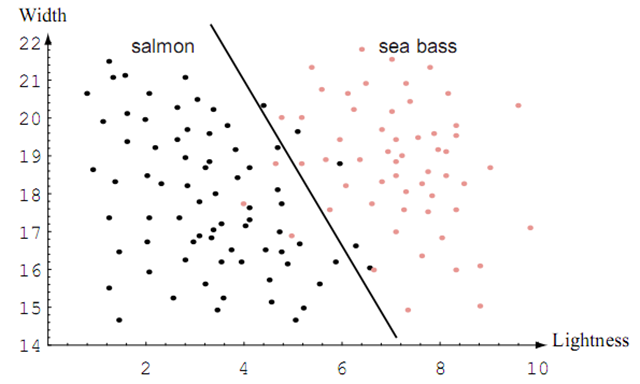
\includegraphics[width=\textwidth]{decision_boundary_linear}
        \label{fig:decision_boundary_linear}
    \end{minipage}
    ~ % space
    \begin{minipage}{0.48\textwidth}
        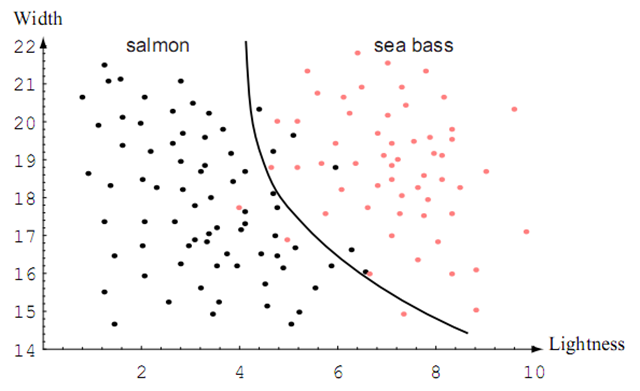
\includegraphics[width=\textwidth]{decision_boundary_smooth}
        \label{fig:decision_boundary_smooth}
    \end{minipage}
    \caption[Fronteira de decisão no espaço de características 2-dimensional]{Fronteira de decisão no espaço de características 2-dimensional de amostras de pele e não pele do conjunto de dados SFA. Os eixos representam os canais a e b do modelo de cores Lab. As figuras à esquerda e à direita mostram a separação do espaço de características por funções linear e não linear, respectivamente. Vale ressaltar que, a complexidade computacional aumenta significativamente nos casos em que existem muitas características. Fonte: proposto pelo autor.}
    \label{fig:decision_boundary}
\end{figure}

Note que a fronteira de decisão é uma função hipotética que o algoritmo de aprendizado deve produzir com base no treinamento dos dados. Ela deve ser mais próxima possível de uma função alvo ou função objetivo $f : X\mapsto Y$ que é desconhecida \citep{mostafa:12}.

Este tipo de abordagem é caracterizada como aprendizagem supervisionada, ou seja, os dados de treinamento contêm amostras explícitas de como deve ser a saída correta sobre um vetor de entrada \citep{mostafa:12}.

Na aprendizagem não supervisionada, também conhecida como clusterização, não se sabe a que classes pertencem os dados de treinamento. A missão do classificador, neste caso, é aglomerar os dados de entrada em agrupamentos naturais \citep{duda:12}. Logo, a aprendizagem não supervisionada pode ser vista como uma tarefa de encontrar padrões ou estruturas espontaneamente a partir dos dados de entrada \citep{mostafa:12}.

Uma outra abordagem é a aprendizagem reforçada que, da mesma forma que na aprendizagem não supervisionada, não usa dados de entrada rotulados, em vez disso, a saída proposta pelo treinamento é utilizada juntamente com uma medida de sua qualidade para melhorar os resultados do classificador \citep{mostafa:12}.

Ainda sobre os resultados do classificador, é importante salientar que aprender os parâmetros de uma função alvo e testá-la nos mesmos dados é um erro fundamental, pois o modelo repetiria os rótulos das amostras tão logo treinadas implicando em um ajuste perfeito dos dados, porém, não seria suficiente para prever qualquer coisa útil sobre novos dados de entrada. Este fenômeno é chamado de sobreajuste e para evitá-lo, o conjunto de dados é, então, particionado de forma a armazenar parte dos dados para uma etapa subsequente de teste, no intuito de encontrar o estimador com a melhor performance \citep{mostafa:12}.

A divisão dos dados em subconjuntos disjuntos de treinamento e de teste é uma abordagem eficaz quando uma grande quantidade de dados está disponível. Entretanto, quando os dados são limitados, a retenção de parte deles para o conjunto de teste reduz ainda mais o número de amostras disponíveis para treinamento \citep{mitchell:97}. Logo, uma outra abordagem, conhecida como validação cruzada, pode ser aplicada de modo que todo o conjunto de dados é usado no treinamento e teste.

A validação cruzada\index{cruzada!validação} consiste em dividir o conjunto de dados $D$ em $K$ subconjuntos disjuntos $D_1, D_2, \ldots, D_K$, onde cada subconjunto tem tamanho aproximado $N/K$. O modelo é, então, treinado em cada um desses subconjuntos, exceto um que é mantido como um conjunto de validação, no qual a medida de erro é realizada. Este processo é repetido $K$ vezes, de tal forma que cada um dos subconjuntos tem a oportunidade de agir como o conjunto de teste e, por isso, essa abordagem também é conhecida como \emph{K-fold}. Ao final de todas as $K$ iterações, a média do erro obtido por cada estimador é usado como a medida de performance do classificador \citep{mostafa:12}.

Alguns dos classificadores, que foram usados nos experimentos preliminares do capítulo \ref{cap:experimentos}, serão brevemente tratados nas seções \ref{sec:clasificadores_svm} e \ref{sec:clasificadores_knn}.


%% ------------------------------------------------------------------------- %%
\subsection{Máquinas de vetores suporte}
\label{sec:clasificadores_svm}
As Máquinas de Vetores Suporte (SVM) constituem uma técnica de aprendizagem computacional baseada na Teoria de Aprendizado Estatístico \citep{vapnik:13}, cujo objetivo era de resolver problemas de classificação de padrões. Na prática, uma SVM tem a habilidade de gerar um hiperplano ou conjunto de hiperplanos num espaço de alta ou infinita dimensionalidade, que pode ser usado para tarefas de classificação, regressão ou outras \citep{duda:12}.

Derivado do próprio nome da técnica, os vetores de suporte são as amostras do conjunto de treinamento que definem o hiperplano ótimo e são os padrões mais difíceis de classificar \citep{duda:12}. Intuitivamente, eles são os padrões mais relevantes para a tarefa de classificação, pois uma mudança nestes vetores implicam diretamente no resultado do hiperplano ótimo \footnote{O hiperplano de separação ótimo de uma SVM é aquele de uma classe de hiperplanos com a maior margem de separação entre os dois conjuntos de treinamento \citep{cortes:95}.}.

Seja o conjunto de dados de treinamento com $N$ amostras da forma:
\begin{equation}
\label{eq:svm_dataset}
    D = (x_1, y_1), (x_2, y_2), \ldots, (x_N, y_N)
\end{equation}
\noindent onde cada $x_i$ é um vetor $d$-dimensional da forma dada em \ref{eq:vetor_caracteristicas}, $i = 1, 2, \ldots, N$, $y_i \in Y$ e $Y = \{+1, -1\}$. Portanto, o conjunto de treinamento contém $N$ observações com suas respectivas classes.

Assumindo que $D$ é linearmente separável, pode-se separar os dados por meio de um hiperplano usando um classificador, também linear, definido pela equação \citep{lorena:03}:
\begin{equation}
\label{eq:svm_hyperplano_otimo}
w \cdot x + b = 0
\end{equation}
\noindent onde $w \cdot x$ é um produto escalar, $w$ é o vetor normal ao hiperplano e $b$ é um termo compensador. O parâmetro $\ffrac{b}{||w||}$ determina o deslocamento do hiperplano em relação à origem.

A partir dessa definição, outros dois hiperplanos paralelos ao hiperplano ótimo podem ser obtidos, conforme as equações em \ref{eq:svm_hyperplanos_paralelos}, de forma que uma região delimitada, conhecida como margem, se forma entre eles.

\begin{equation}
\label{eq:svm_hyperplanos_paralelos}
\begin{cases}
    w \cdot x + b = +1\\
    w \cdot x + b = -1
\end{cases}
\end{equation}

Além disso, algumas restrições são definidas para evitar que não existam pontos entre $w \cdot x + b = 0$ e $w \cdot x + b = \pm 1$, formalmente tem-se \citep{lorena:03}:
\begin{equation}
\label{eq:svm_hyperplanos_paralelos_restricoes}
\begin{cases}
    w \cdot x_i + b \geq +1, & \text{se}\ y_i = +1\\
    w \cdot x_i + b \leq -1, & \text{se}\ y_i = -1
\end{cases}
\end{equation}
\noindent ou, equivalentemente:
\begin{equation}
\label{eq:svm_hyperplanos_paralelos_restricoes_equiv}
    y_i (w \cdot x_i + b) \geq 1
\end{equation}

Segundo \citet{campbell:00}, no sistema dado na equação \ref{eq:svm_hyperplanos_paralelos_restricoes}, supõe-se que a margem é sempre maior que a distância entre $w \cdot x + b = 0$ e $|w \cdot x + b = 1|$ e, por essa razão, SVMs desta natureza são usualmente denominadas de SVMs com margens rígidas. A figura~\ref{fig:svm_support_vectors} mostra a representação gráfica destes conceitos.

\begin{figure}[!h]
  \centering
  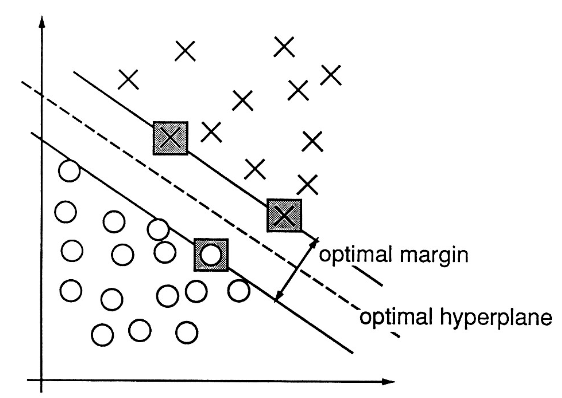
\includegraphics[width=.5\textwidth]{svm_support_vectors}
  \caption[Exemplo de um problema de classes binárias separáveis num espaço $2$-dimensional]{Exemplo de um problema de classes binárias separáveis num espaço $2$-dimensional. Os vetores de suporte, marcados com quadrados cinza, definem a margem de maior separação entre as duas classes. Fonte: \citet{cortes:95}.}
  \label{fig:svm_support_vectors}
\end{figure}

Geometricamente, a distância entre os dois hiperplanos paralelos ao hiperplano ótimo é $\ffrac{2}{||w||}$. Consequentemente, pode-se deduzir que a distância entre o hiperplano ótimo e $w \cdot x + b = \pm 1$ é $\ffrac{1}{||w||}$. Portanto, a minimização de $||w||$ maximiza a margem e, sendo assim, tem-se um problema de otimização no qual deseja-se minimizar $||w||^2$ sujeito às restrições em \ref{eq:svm_hyperplanos_paralelos_restricoes_equiv} \citep{lorena:03}. Logo, $w$ e $b$ ótimos que resolvem este problema definem o classificador e podem ser obtidos por multiplicadores de Lagrange \citep{campbell:00}:
\begin{equation}
\label{eq:svm_margens_rigidas}
\text{Maximizar: } \sum_{i=1}^N \alpha_i - \frac{1}{2} \sum_{i, j=1}^N \alpha_i \alpha_j y_i y_j x_i\cdot x_j
\end{equation}

\begin{equation}
\label{eq:svm_margens_rigidas_restricoes}
\text{Sujeito a: }
\begin{cases}
    \alpha_i \geq 0\\[1em]
    \sum_{i=1}^N \alpha_i y_i = 0
\end{cases}
\end{equation}
\noindent onde $\alpha$ são os multiplicadores de Lagrange.

É importante ressaltar que este tipo de SVM tem êxito em conjuntos de dados de treinamento linearmente separáveis. Nos casos em que os dados são não linearmente separáveis, é admitida a ocorrência de alguns erros de classificação para o conjunto de treinamento, pela inclusão de variáveis de relaxamento \citep{lorena:03}. Essas alterações foram produzidas por \citet{cortes:95} e fazem parte de uma técnica denominada suavização de margens e, por conseguinte, SVMs dessa família também são chamadas de SVM com margens suaves. Logo, o problema de otimização torna-se \citep{lorena:03}:
\begin{equation}
\label{eq:svm_margens_suaves_def}
\text{Minimizar: } ||w||^2 + C\sum_{i=1}^N \xi_i
\end{equation}

\begin{equation}
\label{eq:svm_margens_suaves_def_restricoes}
\text{Sujeito a: }
\begin{cases}
    \xi_i \geq 0\\[1em]
    y_i (w \cdot x_i + b) \geq 1 - \xi_i
\end{cases}
\end{equation}
\noindent onde $C$ é uma constante de regularização determinada empiricamente que impõe um peso diferente para o treinamento em relação à generalização. Sendo assim, o problema pode ser resolvido da mesma maneira com a equação em \ref{eq:svm_margens_rigidas}, porém, com algumas alterações nas restrições \citep{lorena:03}:

\begin{equation}
\label{eq:svm_margens_suaves_restricoes}
\text{Sujeito a: }
\begin{cases}
    0 \leq \alpha_i \leq C\\[1em]
    \sum_{i=1}^N \alpha_i y_i = 0
\end{cases}
\end{equation}

Em geral, a maioria dos problemas de classificação impedem que classificadores lineares sejam utilizados por não ser possível obter resultados satisfatórios na partição dos dados de treinamento por um hiperplano. Entretanto, as SVMs lineares podem ser estendidas para lidar com essa situação mapeando o espaço de entrada em um espaço de características de dimensão mais alta, tipicamente muito maior que o espaço original \citep{duda:12}, da forma:
\begin{equation}
\label{eq:svm_dataset_transformado}
    D' = (\Phi(x_1), y_1), (\Phi(x_2), y_2), \ldots, (\Phi(x_N), y_N)
\end{equation}

A escolha apropriada de uma função $\Phi$ torna o conjunto de treinamento linearmente separável no espaço transformado \citep{lorena:03}. A forma do hiperplano ótimo agora é definida por:
\begin{equation}
\label{eq:svm_hyperplano_otimo_trasnformado}
w \cdot \Phi(x) + b = 0
\end{equation}

Logo, os conceitos de vetores de suporte, margem, hiperplanos paralelos e, consequentemente, de problema de otimização para encontrar a solução para os parâmetros $w$ e $b$ se aplicam aqui de forma similar. Formalmente, o problema de otimização pode ser resolvido como \citep{lorena:03}:
\begin{equation}
\label{eq:svm_nao_linear}
\text{Maximizar: } \sum_{i=1}^N \alpha_i - \frac{1}{2} \sum_{i, j=1}^N \alpha_i \alpha_j y_i y_j \Phi(x_i)\cdot \Phi(x_j)
\end{equation}
\noindent sujeito às mesmas restrições definidas em \ref{eq:svm_margens_suaves_restricoes}.

Agora, há a necessidade de se definir como o produto interno $\Phi(x_i)\cdot \Phi(x_j)$ entre dois vetores quaisquer $x_i, x_j \in D$ é realizado, cuja resposta está na introdução do conceito de \emph{kernels} \citep{lorena:03}.

\emph{Kernels} são funções\index{\emph{kernel}!funções} que têm a finalidade de projetar os vetores de entrada num espaço de características com número de dimensões exponencial ou infinito \citep{taylor:04}, da forma:
\begin{equation}
\label{eq:svm_kernels}
k(x_i, x_j) =  \Phi(x_i) \cdot \Phi(x_j)
\end{equation}

Logo, é possível aplicar um \emph{kernel} como descrito na equação \ref{eq:svm_kernels} na etapa de otimização da SVM, calculando de maneira eficiente o produto interno a partir dos dados de entrada, sem nem mesmo computar explicitamente o mapeamento da função $\Phi$ \citep{taylor:04}.

Alguns dos \emph{kernels} mais utilizados são \citep{lorena:03}:
\begin{enumerate}[label=(\roman*)]
\item \emph{Kernel} linear\index{\emph{kernel}!linear}
\begin{equation}
\label{eq:svm_kernel_linear}
k(x_i, x_j) =  (x_i \cdot x_j)
\end{equation}
O \emph{kernel} linear é o mais simples das funções \emph{kernel} e se dá pelo produto interno de dois vetores $x_i$ e $x_j$.

\item \emph{Kernel} polinomial\index{\emph{kernel}!polinomial}
\begin{equation}
\label{eq:svm_kernel_polinomial}
k(x_i, x_j) =  ({\gamma x_i \cdot x_j + r} )^g
\end{equation}
\noindent onde $g$ é o grau do polinômio e $r$ é um termo constante. Para este \emph{kernel}, os mapeamentos $\Phi$ também são funções polinomiais e, portanto, a complexidade é proporcional à escolha de $g$ \citep{lorena:03}.

\item \emph{Kernel} gaussiano\index{\emph{kernel}!gaussiano ou RBF}
\begin{equation}
\label{eq:svm_kernel_rbf}
k(x_i, x_j) =  \exp{\big(-\gamma {||x_i - x_j||}^2 \big)}
\end{equation}
Também conhecido como Função de Base Radial (RBF), o \emph{kernel} gaussiano corresponde a um espaço de características de dimensão infinita \citep{lorena:03}.
\end{enumerate}

No \emph{kernel} RBF e polinomial, o parâmetro $\gamma$ pode ser visto como o inverso do raio de influência das amostras selecionadas pelo modelo como vetores de suporte \citep{scikit-learn:11}.

%% ------------------------------------------------------------------------- %%
\subsection{\emph{k}-vizinhos mais próximos}
\label{sec:clasificadores_knn}
O $k$-Vizinhos Mais Próximos ($k$-NN) é um algoritmo baseado em instâncias, o que significa que a função alvo não é aprendida com base em amostras de treinamento; elas simplesmente são mantidas, de maneira que a relação entre uma nova amostra com as amostras de treinamento armazenadas é avaliada e uma função alvo é, então, atribuída a ela \citep{mitchell:97}.

Como o próprio nome sugere, o $k$-NN classifica um novo ponto $x$ atribuindo-lhe a classe de maior frequência dentre as $k$ amostras mais próximas, ou seja, a decisão da classe de $x$ é feita por maioria de votos dos $k$ vizinhos mais próximos e, por essa razão, é interessante que a escolha de $k$ seja um número ímpar para evitar empates \citep{duda:12}.

\begin{figure}[!h]
  \centering
  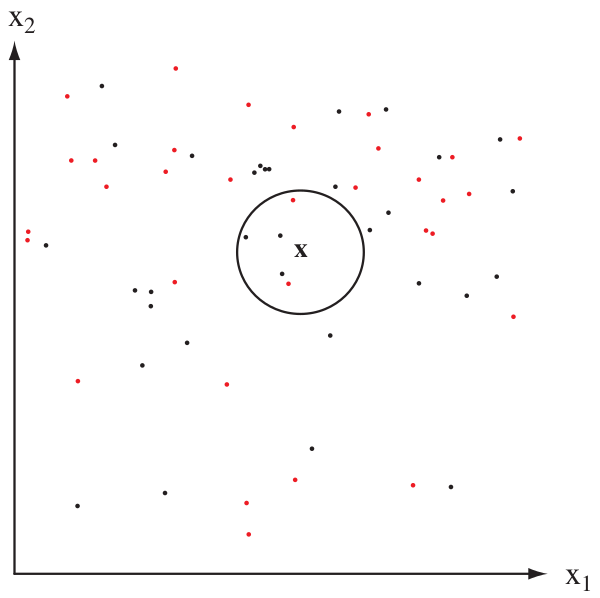
\includegraphics[width=.65\textwidth]{knn_exemplo}
  \caption[Exemplo de aplicação do $k$-NN na tarefa de classificação num espaço $2$-dimensional]{Exemplo de aplicação do k-NN na tarefa de classificação num espaço $2$-dimensional. O algoritmo avalia as $k$ amostras próximas de $x$, criando uma região esférica, e rotula $x$ com a classe de maior frequência. Neste caso, $k = 5$ e a classe atribuída a $x$ deve ser a mesma dos pontos em azul. Fonte: proposto pelo autor.}
  \label{fig:knn_exemplo}
\end{figure}

Seja $D$ o conjunto de dados de treinamento com $N$ amostras da forma apresentada em \ref{eq:svm_dataset}. Logo, a distância entre duas amostras $x_i$ e $x_j$ quaisquer pode ser obtida em termos da distância Euclidiana, definida como:

\begin{equation}
\label{eq:knn_distancia_euclidiana}
d(x_i, x_j) = \sqrt{\sum_{r=1}^d (a_r(x_i) - a_r(x_j))^2}
\end{equation}
\noindent onde $a_r$ refere-se ao $r$-ésimo atributo do vetor de entrada $x$ e $i, j = 1, 2, \ldots, N$. Outras métricas de distância podem ser atribuídas a $d(x_i, x_j)$, tais como, Manhattan, Chebyshev e Minkowski \citep{duda:12}.

Para, então, classificar uma nova amostra $x_q$, toma-se $x_1, \ldots, x_k$ instâncias do conjunto de treinamento, cujas distâncias dadas por \ref{eq:knn_distancia_euclidiana}, são dos $k$ pontos mais próximos de $x_q$. Sendo assim, a função que estima a classe de $x_q$ é dada por \citep{mitchell:97}:
\begin{equation}
\label{eq:knn_funcao_argmax}
g(x_q) \gets \argmax_{y \in Y} \sum_{i=1}^k \delta (y, f(x_i))
\end{equation}
\noindent onde
\begin{equation}
\label{eq:knn_delta}
  \delta (y, f(x_i)) =  \begin{cases}
                1, \quad \text{se}\ y = f(x_i) \\
                0, \quad \text{caso contrário}
              \end{cases}
\end{equation}

É importante ressaltar que $f(x_i)$ é conhecida, ou seja, é a classe da amostra $x_i$ do conjunto de treinamento.

Uma variação óbvia da função dada na equação \ref{eq:knn_funcao_argmax} é a atribuição de pesos de cada um dos $k$ vizinhos, conforme sua distância, para um ponto $x_q$ sendo classificado \citep{mitchell:97}. Essa variação implica que pontos mais próximos de $x_q$ têm maior influência na sua rotulação. Formalmente, tem-se que \citep{mitchell:97}:
\begin{equation}
\label{eq:knn_funcao_argmax_pesos}
g(x_q) \gets \argmax_{y \in Y} \sum_{i=1}^k w_i \delta (y, f(x_i))
\end{equation}
\noindent onde
\begin{equation}
\label{eq:knn_funcao_peso}
  w_i = \frac{1}{d(x_q, x_i)^2}
\end{equation}

No caso em que $d(x_q, x_i) = 0$, ou seja, $x_q$ e $x_i$ estão exatamente nas mesmas coordenadas, $g(x_q)$ pode assumir o mesmo valor de $f(x_i)$. Se há outras amostras de treinamento $x_i$ com a mesma característica, então $x_q$ pode assumir a classe da maioria delas \citep{mitchell:97}.


%% ------------------------------------------------------------------------- %%
\subsection{Árvores de decisão}
\label{sec:clasificadores_arvores_decisao}
Árvore de decisão é um método para aproximação de funções alvo discretas, nas quais a função aprendida é representada por uma árvore de decisão ou, ainda, por um conjunto de regras do tipo \emph{Se-Então} que são de fácil interpretação. É uma das técnicas de aprendizagem mais populares de inferência indutiva\footnote{A tarefa de indução é desenvolver uma regra de classificação que pode determinar a classe de qualquer objeto a partir dos valores de seus atributos \citep{quinlan:86}.} \citep{mitchell:97}.

As amostras de um conjunto de dados são classificadas por uma árvore de decisão por um processo iterativo onde um atributo (nó) é escolhido como raiz até algum nó folha, onde a classe é atribuída à amostra. Cada ramo partindo de um nó representa um dos valores possíveis de um dado atributo \citep{mitchell:97}.

Há uma família de algoritmos de árvore de decisão. Um deles é o Divisor Iterativo 3 (ID3) proposto por \citet{quinlan:86}. O ID3 avalia cada atributo através de um teste estatístico para determinar o quão bem ele, por si só, classifica as amostras de treinamento. O melhor atributo é selecionado como o nó raiz da árvore. Um ramo descendente do nó raiz é criado para cada valor possível deste atributo e as amostras de treinamento são classificadas para o nó descendente adequado. Este processo é então repetido recursivamente utilizando as amostras associadas a cada nó descendente. Esse é um algoritmo de busca guloso, já que ele não retrocede para reconsiderar escolhas anteriores \citep{mitchell:97}. O algoritmo para quando o subconjunto de amostras associado a um nó é da mesma classe ou quando não há relevância estatística para uma nova partição \citep{quinlan:86}.

Para medir a impureza de uma partição, o ID3 usa o conceito de entropia, formalmente \citep{quinlan:86}:

\begin{equation}
\label{eq:arvore_devisao_entropia}
H(D) = - y_\oplus log_2 y_\oplus - y_\ominus log_2 y_\ominus
\end{equation}
\noindent onde $D$ é o conjunto de dados de treinamento com $N$ amostras da forma apresentada em \ref{eq:svm_dataset}, $y_\oplus$ e $y_\ominus$ é a proporção de amostras positivas e negativas de $D$, respectivamente. É importante notar que a entropia é 0 quando todas as amostras de $D$ pertencem à mesma classe, 1 quando $D$ contém um número igual de amostras positivas e negativas e um valor entre 0 e 1 nos demais casos \citep{mitchell:97}.

Dada a entropia como uma medida de impureza de um conjunto de amostras de treinamento, pode-se definir o teste estatístico, conhecido como ganho de informação, que mede a efetividade de um atributo na classificação dos dados de treinamento, formalmente \citep{quinlan:86}:
\begin{equation}
\label{eq:arvore_devisao_ganho_informacao}
IG(D, a_r) = H(D) - \sum_{v \in V(a_r)} \frac{|D_v|}{|D|} H(D_v)
\end{equation}
\noindent onde $V(a_r)$ é o conjunto de todos os possíveis valores do atributo $a_r$, $D_v$ é o subconjunto de $D$ no qual o atributo $a_r$ tem o valor $v$.

Vale enfatizar que o primeiro termo da equação dado em \ref{eq:arvore_devisao_ganho_informacao} é a entropia do conjunto original $D$ e o segundo termo é o valor esperado da entropia depois que $D$ é particionado usando o atributo $a_r$ \citep{mitchell:97}. Outro aspecto importante é que o algoritmo inicia com o conjunto $D$ original, que é substituído por $D_v$ à medida que a recursão se aprofunda.

Batizado de C4.5, \citet{quinlan:93} estendeu o ID3 para possibilitar o uso de atributos contínuos, atributos com dados ausentes e melhoria na eficiência computacional. Além disso, essa versão cuida de questões como quão profunda a árvore deve ser para evitar que os dados de treinamento sejam perfeitamente classificados, ou seja, quando o conjunto de treinamento é particionado até que cada subconjunto contenha apenas amostras de uma única classe. A estratégia adotada por \citet{quinlan:93} foi podar a árvore posteriormente à geração da árvore ajustada. Esse processo, apesar de ser mais lento que a proposta anterior do ID3, tornou o algoritmo mais confiável e com maior capacidade de generalização.


%% ------------------------------------------------------------------------- %%